\chapter{Methodology}
\label{chap:methodology}

\section{Point Cloud Data}
\label{sec:point_cloud_data}

This project aims to work with large amounts of point cloud data. It contains arrays of three-dimensional coordinates and the four-component color data. The color information does not affect performance strongly. However, the massive number of points itself introduces the heavy load on processor resources. For improving the performance of visualization software, this work proposes two methods: Generating Levels of Detail (LODs) and Creating a heightmap.


\section{Data Preprocessing}
\label{sec:data_preprocessing}

The data itself is stored in a PCAP file as captured packet stream from the lidar. It is necessary to preprocess original files before working on the point cloud. The preprocessing involves three main steps: converting the file from PCAP format to the LAS format, importing the LAS file into Unity, and splitting the point cloud data into chunks.

\subsection{Converting to LAS format}
\label{subsec:converting_to_las}

PCAP is an open network traffic capturing system that uses its own \texttt{.pcap} file format [citation here]. As mentioned above, the file contains the recorded packet stream from the lidar at the time of capturing the area. It means that the data is stored as individual captures from various perspectives and at different times.
This step collects the data stream into the single point cloud, which represents the whole captured area. The resulting point cloud is stored in LAS format [citation here].
The VeloView is a software for previewing the data from lidars and converting it to different formats [citation here]. It is used to preview the PCAP stream and convert it to the LAS format for further processing.

\subsection{Importing LAS files into Unity}
\label{subsec:importing_las_unity}

As this project uses the Unity engine as a base, it is essential to have the ability to read LAS files within its programming environment. Importing the LAS file into Unity is being done with the help of the LASzip.NET library.
LASzip is a library for compressing, decompressing, and parsing the lidar data from LAS files [citation here]. LASzip.NET is a wrapper for LASzip which makes it possible to utilize the functionality of the main library within the .NET environment which in turn is being used for programming in the Unity engine.

\subsection{Splitting into chunks}
\label{subsec:splitting_into_chunks}

For the proposed methods it is crucial to split the point cloud into smaller units (chunks) that are easier to process. It also helps to process the data in a parallel manner, thereby making the algorithms more scalable in terms of performance.

In terms of the given project, the chunk is a space bounded by computed borders. It has a position, and a size, which is the same for its width, height, and depth. 

\paragraph{Algorithm}
At the start, the algorithm computes the number of chunks in three dimensions using the formula \ref{formula:n_chunks}. It uses the predefined chunk size and the boundaries of the point cloud object.

The number of chunks for an axis $\alpha$ is computed as follows:

\begin{equation}
\label{formula:n_chunks}
N_{chunks}^\alpha = \lceil BBox_{max}^\alpha - BBox_{min}^\alpha \rceil / Size_{chunk}
\end{equation}

For that, the chunk grid will have the size of $N_{chunks}^X \times N_{chunks}^Y \times N_{chunks}^Z$.

The chunks are stored in a three-dimensional array. It means that each chunk has its corresponding index.

After that, the algorithm iterates overall points and computes the exact chunk index they correspond to, based on their global position.

The chunk index for a point with position $pos$ on an axis $\alpha$ is computed as shown on formula \ref{formula:point_index}:

\begin{equation}
\label{formula:point_index}
Index_{pos}^\alpha = \left \lfloor \frac{pos^{\alpha} - BBox_{min}^\alpha}{Size_{chunk}} \right \rfloor
\end{equation}

In the end, the points are stored within chunks. It is now possible to read the point cloud data in chunks.


\section{Method 1: Generating LODs}
\label{sec:generating_lods}

The level of detail defines the complexity of the model [citation here]. For this project, the level of detail adjusts the number of points shown for a particular object.

The LOD of L shows L\% of all points of an object. For example, a chunk with LOD 100 renders all its points while LOD 70 renders 70\% of chunk points. The algorithm does this by introducing the render probability.

\begin{equation}
\label{formula:render_probability}
P_{Render} = \frac{LOD}{100}
\end{equation}

The first approach is to generate different levels of detail for each chunk so it will be possible to show fewer points for chunks that are far enough not to notice the low-detailed chunk.


\section{Method 2: Creating a Mesh}
\label{sec:creating_mesh}

\begin{figure}[ht]
    \centering
    
    \begin{subfigure}[t]{0.4\textwidth}
        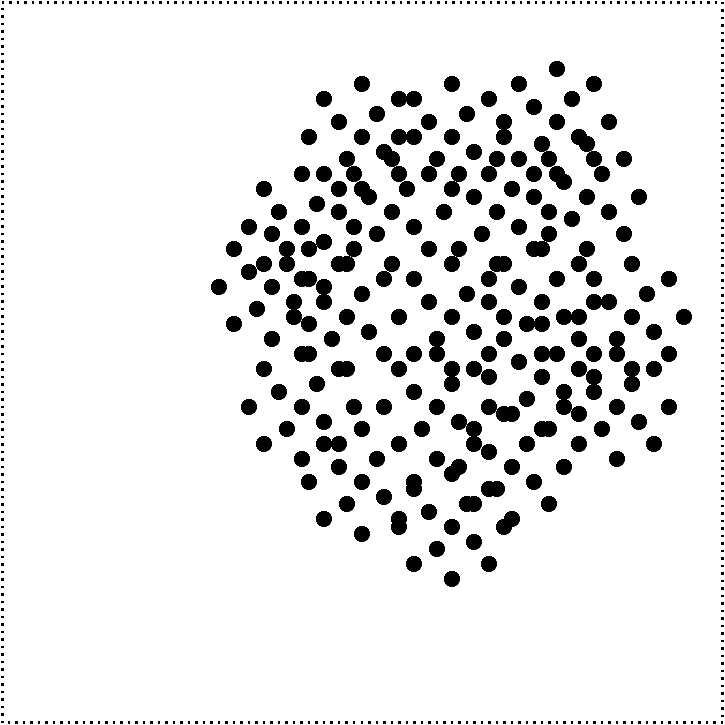
\includegraphics[width=\textwidth]{figs/implementation/point-cloud-plot.pdf}
        \caption{Example of point cloud data in two dimensions.}
    \end{subfigure}
    % side-to-side
    \begin{subfigure}[t]{0.4\textwidth}
        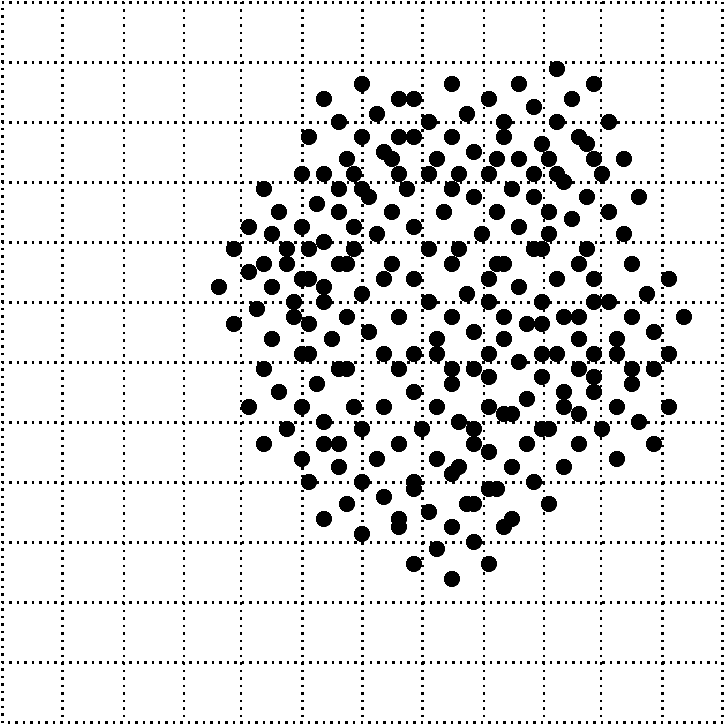
\includegraphics[width=\textwidth]{figs/implementation/occurrence-grid.pdf}
        \caption{Occurrence grid.}
    \end{subfigure}
    
    \begin{subfigure}[t]{0.5\textwidth}
        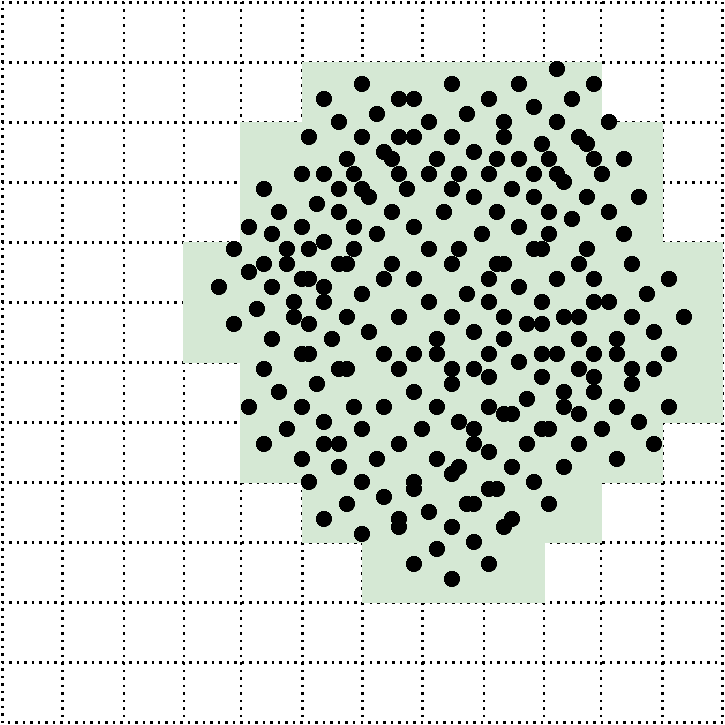
\includegraphics[width=\textwidth]{figs/implementation/occurrence-map-applied.pdf}
        \caption{Applied occurrence map.}
    \end{subfigure}
    
    \caption{Applying occurrence map.}
    \label{fig:occurrence_map}
\end{figure}
